%!TEX program = xelatex
\documentclass[UTF8,zihao=5]{ctexart} %ctex包的article


\usepackage[hidelinks]{hyperref}%超链接,自动加到目录里面



\title{{\bfseries\rmfamily\Huge{高等流体力学\hspace{1em}\\第2次阅读报告}}}
\author{周涵宇 2022310984}
\date{}

\usepackage[a4paper]{geometry}
\geometry{left=0.75in,right=0.75in,top=1in,bottom=1in}%纸张大小和页边距

\usepackage[
UseMSWordMultipleLineSpacing,
MSWordLineSpacingMultiple=1.5
]{zhlineskip}%office风格的行间距

\usepackage{fontspec}
\setmainfont{Times New Roman}
\setsansfont{Source Sans Pro}
\setmonofont{Latin Modern Mono}
\setCJKmainfont{SimSun}[AutoFakeBold=true]
% \setCJKmainfont{仿宋}[AutoFakeBold=true]
\setCJKsansfont{黑体}[AutoFakeBold=true]
\setCJKmonofont{DengXian}[AutoFakeBold=true]

\setCJKfamilyfont{kaiti}{楷体}
\newfontfamily\CM{Cambria Math}


% \usepackage{indentfirst} %不工作 怎样调整ctex的段首缩进大小呢

\usepackage{fancyhdr}
\pagestyle{fancy}
\lhead{
    \CJKfamily{kaiti}{
        高等流体力学作业\hspace{6em}
        班级\ \ 航博221\hspace{6em}
        学号\ \ 2022310984\hspace{6em}
        姓名\ \ 周涵宇
        }
}
\chead{}
\rhead{}
\lfoot{}
\cfoot{\thepage}
\rfoot{}
\renewcommand{\headrulewidth}{0.5pt} %改为0pt即可去掉页眉下面的横线
\renewcommand{\footrulewidth}{0pt} %改为0pt即可去掉页脚上面的横线
\setcounter{page}{1}


% \usepackage{bm}

\usepackage{amsmath,amsfonts}
\usepackage{array}
\usepackage{enumitem}
\usepackage{unicode-math}

% \usepackage{titlesec} % it subverts the ctex titles
\usepackage{titletoc}


% titles in toc:
\titlecontents{section}
              [2cm]
              {\sffamily\zihao{5}\mdseries}%
              {\contentslabel{3em}}%
              {}%
              {\titlerule*[0.5pc]{-}\contentspage\hspace*{1cm}}

\titlecontents{subsection}
              [3cm]
              {\rmfamily\mdseries\zihao{5}}%
              {\contentslabel{3em}}%
              {}%
              {\titlerule*[0.5pc]{-}\contentspage\hspace*{1cm}}

\titlecontents{subsubsection}
              [4cm]
              {\rmfamily\mdseries\zihao{5}}%
              {\contentslabel{3em}}%
              {}%
              {\titlerule*[0.5pc]{-}\contentspage\hspace*{1cm}}
\renewcommand*\contentsname{\hfill \sffamily\mdseries 目录 \hfill}

\ctexset{
    section={   
        % name={前面,后面},
        number={\arabic{section}.},
        format=\sffamily\raggedright\zihao{4}\mdseries,
        indent= {0em},
        aftername = \hspace{0.5em},
        beforeskip=1ex,
        afterskip=1ex
    },
    subsection={   
        % name={另一个前面,另一个后面},
        number={\arabic{section}.\arabic{subsection}.}, %如果只用一个数字而非1.1
        format=\rmfamily\raggedright\mdseries\zihao{5},%正体字体,不加粗,main字体,五号字
        indent = {2em}, %缩进
        aftername = \hspace{0.5em},
        beforeskip=1ex,
        afterskip=1ex
    },
    subsubsection={   
        % name={另一个前面,另一个后面},
        number={\arabic{section}.\arabic{subsection}.\arabic{subsubsection}.}, %默认的 1.1.1
        format=\rmfamily\raggedright\mdseries\zihao{5},%无衬线字体,加粗,sans字体,五号字
        indent = {2em}, %缩进
        aftername = \hspace{0.5em},  %名字和标题间插入字符(此处是空白)
        beforeskip=1ex, %空行
        afterskip=1ex
    }
}

\usepackage{float}
\usepackage{graphicx}
\usepackage{multirow}
\usepackage{multicol}
\usepackage{caption}
\usepackage{subcaption}
\usepackage{cite}


%part、section、subsection、subsubsection、paragraph、subparagraph
\newcommand{\bm}[1]{{\mathbf{#1}}}
\newcommand{\trans}[0]{^\mathrm{T}}
\newcommand{\tran}[1]{#1^\mathrm{T}}
\newcommand{\hermi}[0]{^\mathrm{H}}
\newcommand{\conj}[1]{\overline{#1}}
\newcommand*{\av}[1]{\left\langle{#1}\right\rangle}
\newcommand*{\avld}[1]{\frac{\overline{D}#1}{Dt}}
\newcommand*{\pd}[2]{\frac{\partial #1}{\partial #2}}
\newcommand*{\pdcd}[3]{\frac{\partial^2 #1}{\partial #2 \partial #3}}
\newcommand*{\inc}[0]{{\Delta}}

\newcommand*{\uu}[0]{\bm{u}}
\newcommand*{\vv}[0]{\bm{v}}
\newcommand*{\g}[0]{\bm{g}}
\newcommand*{\nb}[0]{{\nabla}}



\begin{document}

\maketitle
\thispagestyle{fancy}


% \begin{center}
%     \rmfamily
%     \tableofcontents\setcounter{page}{0}
% \end{center}
% \thispagestyle{empty} % 目录
% \newpage %换页

阅读文献:A bulk-interface correspondence for equatorial waves\cite{tauber2019bulk}
(赤道波的体-界面相似性)。


\section{研究背景和意义}

目前,凝聚态物理中发展的一些拓扑工具正在辅助流体波动的研究,
包括微流体\cite{souslov2017topological},
声波\cite{yang2015topological},
行星大气\cite{delplace2017topological,vallis2017atmospheric},
还有活性物质流动\cite{shankar2017topological}的研究。
研究认为,无界几何上线性算子的特征模态包含了许多频谱的信息,
这些信息是重要且鲁棒的。
这些信息体现在闭曲面上参数化特征模态的弯曲。
这种弯曲代表一个拓扑不变量,称其为Chern数,可以被显式计算出来。
例如,Delplace\cite{delplace2017topological}表明,
旋转浅水模型的惯性-重力波在$(k_x,k_y,f)$空间中有这样的拓扑特性,其中
$f$是科里奥利系数,$(k_x,k_y)$是波数。
这个研究中,在正频率的惯性-重力波中,参数空间中,围绕原点有
Chern数等于2的区域,而Chern数在零频率(地转模式)趋于0。

上述奇异性的表现之一是,假设其中一个参数随空间变化,并计算同一个算子的频谱。
Matsuno\cite{matsuno1966quasi},在浅水模型中计算了赤道β面的上述
问题,其中假设经向$y$轴上科里奥利参数的线性分布。
他发现了色散关系中存在两个分支,当纬向$x$波数变化时波动在
赤道Kelvin波和Rossby-重力混合波两个波段之间转换,
现在称之为Yanai波。相比于其他波,这些波更加局限于沿赤道方向且为单方向的。
行星涡量的梯度也支持低频率行星Rossby波作为退化地转模态的抬升部分。
然而,与Kelvin和Yanai波不同的是,Rossby波一直保持在地转模态中。
因此,在赤道β面上,当纬向波数从负值变化到正值时,正频率惯性-重力波
的波段净增加了两个模态\cite{delplace2017topological}。
描述体波退化的拓扑不变量,第一Chern数和赤道β平面不同波段间模态的转移间存在
一定相似性,让人想到Atiyah-Singer指标理论\cite{bal2019continuous,faure2019manifestation},
可称其为拓扑-频谱相似性。这种相似性被证明在理解分子频谱\cite{faure2000topological},
或者密度分层中约束的类Lamb波\cite{perrot2018topological}和其他物理应用
\cite{nakahara2003geometry}中有较大作用。


然而,当界面两侧可以被赋予不同的拓扑指标——而非是在参数空间中
穿越频带的某点时,
或许存在更强的体-界面相似性。
作为界面两侧不同波段拓扑指标不同的结果,
体-界面相似性因而可以预测困在界面中
单方向边界模态的数量。
在凝聚态物理中,由于内在的晶格结构,
体-界面相似性就天然遵循了边界上
单方向边界模态的拓扑指标给出的体-边界相似性\cite{hatsugai1993chern,graf2013bulk}。
在这里,界面相似性其实是由两个拓扑上不同的系统在边界上粘接起来造成的。
因此,自然地,应当探讨是否赤道Kelvin和Yanai波也可以被理解为
两个拓扑上不同的系统的界面状态。
或者说,应当探讨是否每个半球应该被理解成一个独立的拓扑介质。
本文基于Volovik\cite{volovik1988analogue}
和Souslov\cite{souslov2019topological}
的工作,
采用了一个odd viscosity项来在每个半球分别给出一个良定义的拓扑不变量,
并且展现了赤道处的体-界面相似性。

本文使用的线化自转浅水模型组成了一个
可精确求解的、物理相关的模型,并且适用于解释尖锐边界上
当前连续介质中体-界面相似性的问题\cite{bal2019continuous,faure2019manifestation}。
本文的模型同时对赤道波进行了新颖的解读,
将其视作为两个边缘状态在分割两个不同半球的拓扑不同的区域
的界面上的传播。
同时,作为Matsuno\cite{matsuno1966quasi}β面情况的补充,以上
解读也可以给出显式的频谱计算。本文也可以视作Iga\cite{iga1995transition}
关于特征方程中0项守恒的工作的补充。

最后,本文的例子有助于理解流场中更复杂的边界,比如海岸Kelvin波。
在有边界的情况下,Iga\cite{iga1995transition}发现可以通过
改变壁面上的边界条件将海岸Kelvin波从频谱上消除,
这似乎与于其中边界模态的拓扑鲁棒性有所矛盾。
进一步,应当研究这个结论是否在加入odd viscosity之后依然路边\cite{souslov2019topological}.
本文的工作肯定了Iga的结论,这对于流体中体-边相似性的适用性来说是一个悖论。

总体而言,本文的研究是以海洋地理流动为背景,
研究拓扑方法定义出的一种体-面相似性,
通过一个新的简化模型结合odd viscosity的方法研究了
海洋流动中赤道波的一些拓扑特性和界面上的频谱特性,
并且发现了一些情况下体-面相似性失效的问题。

\section{基本模型}


\newcommand{\ee}{{\mathrm e}}
\newcommand{\ii}{{\mathrm i}}
\newcommand{\dd}{{\mathrm d}}

本文的模型是笛卡尔坐标系线化浅水方程中加入额外的大小为$\epsilon$的odd-viscosity项:
\begin{align}
    \partial_t \eta & = - \partial_x u - \partial_y v                         \\
    \partial_t u    & =-\partial_x \eta+ \left(f +\epsilon  \nabla^2 \right)v \\
    \partial_t v    & =-\partial_y \eta- \left(f +\epsilon  \nabla^2 \right)u
\end{align}
其中$u,v$是速度分量,$\eta$是水深增量,$f$是(空间上变化的)科里奥利参数。
上式中时间单位选取使得浅水波相速度$\sqrt{gH}=1$。
通过加入odd-viscosity项可以实现微观层面的时间反演对称性破缺。
这一项对于流动的演化和科里奥利力方向一致,但是大小取决于波数。
文章指出,虽然是无粘的模型,但是由于旋转坐标系下的流体和
传统的情况下不同,在时间反演上是不对称的。
同时,亚格子动力学被认为是与分子运动类似,
因此在模型中需要加入这一项。
本文中,认为$\epsilon$是任意小的常实数,
并在$\epsilon\rightarrow0$的极限验证已知结论。

\section{理论推导}

\subsection{f面中的体波}

给定一个科里奥利参数$f$,在$x,y$平面中讨论波动
问题即为f面近似。
给出模态:
$$
    (\eta,u,v)=(\hat\eta,\hat{u},\hat{v})\exp{[i(\omega t - k_x x - k_y y)]}
$$
则流动系统成为:
\begin{equation}\label{eq:bulk_hamiltonian}
    \omega \begin{pmatrix}
        \hat \eta \\ \hat u \\ \hat v
    \end{pmatrix}=
    \begin{pmatrix}
        0 & k_x & k_y \\ k_x & 0 & -\ii (f-\epsilon  k^2) \\ k_y & \ii (f-\epsilon  k^2) & 0
    \end{pmatrix} \begin{pmatrix}
        \hat \eta \\ \hat u \\ \hat v
    \end{pmatrix}
\end{equation}
其中$k^2=k_x^2 + k_y^2$。可给出特征值:
\begin{equation}\label{eq:omegapm}
    \omega_\pm(k_x,k_y) = \pm \sqrt{k^2 + (f-\epsilon  k^2)^2}, \qquad \omega_0(k_x,k_y) = 0
\end{equation}

图\ref{fig:1}给出了三个特征值的分布,其中有两支分布在正负对称分布。
同时,图\ref{fig:1}给出了特征向量一个分量的分布,在0点都是奇异的。
文章指出了对于$\epsilon\neq0$分量的绝对值大小是不变的,然而对于$\epsilon=0$分量
绝对值是非均匀的。

\begin{figure}[H]
    \centering
    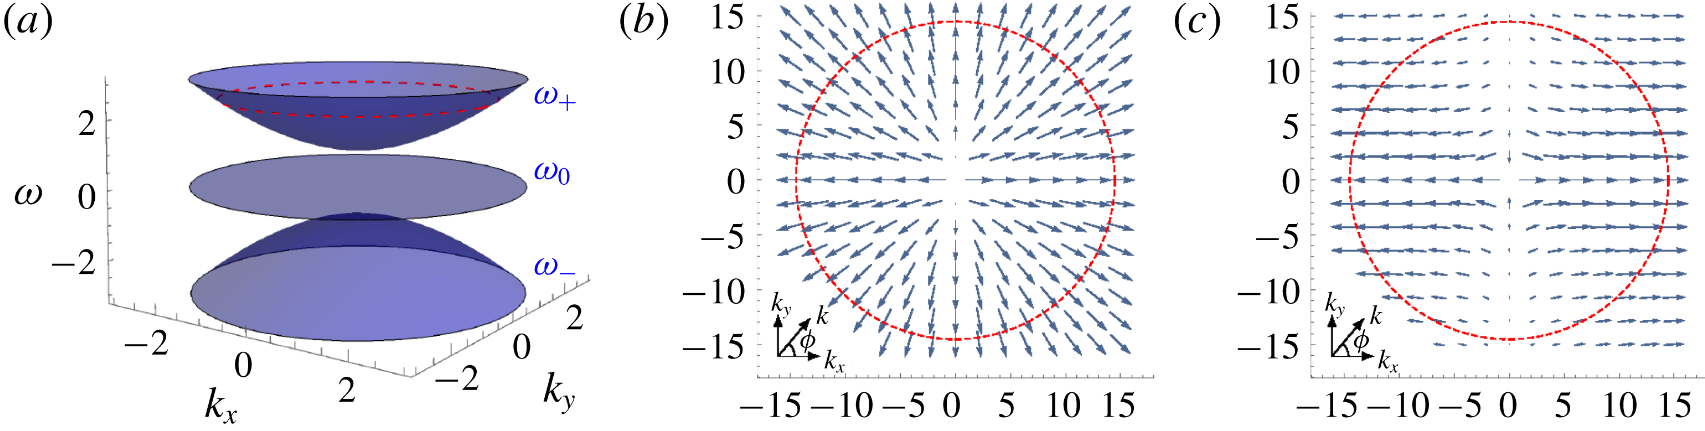
\includegraphics[width=16cm]{fig1.png}  %需调整
    \caption{(a)是三支特征值的分布;(b)是特征向量第二个分量$\hat{u}_+$的分布,$\epsilon=0.2$;
        (c)是(b)在$\epsilon=0$的情况}
    \label{fig:1}
\end{figure}

\subsection{正分支中的拓扑}

文章认为定义\eqref{eq:bulk_hamiltonian}的
相态在空间中每个点是可以定义的。
但是如果在闭曲面上面定义的话,并不保证处处存在光滑的相态。
如果存在奇异性的话,总是可以通过移除一点处
的奇异性使其恢复光滑,但是这个奇异点一定会在闭曲面之外某一点出现。
无法定义全局连续的相态的性质是一个模式的拓扑行为,本文通过一个拓扑指标,
第一Chern数来描述这个事情。
文章中实际上需要在$(k_x,k_y)$平面上研究相态奇异性,
而不是一个闭曲面,因此需要对问题进行紧支化。
因此考虑将无限大平面映射到球面。

首先转换为柱坐标系,$k_x=k\cos{\phi}, k_y=k\sin{\phi}$,
明显可知特征值对$\phi$是不变的。
关于$\omega_{+}$的特征向量标准化后为:
\begin{equation}
    \psi_0(k_x,k_y) = \dfrac{1}{\sqrt{k^2 +(f-\epsilon k^2)^2}} \begin{pmatrix}
        f-\epsilon  k^2 \\ \ii k \sin \phi \\ -\ii k \cos \phi
    \end{pmatrix}
\end{equation}

文章讨论了$k\rightarrow\infty$和$k\rightarrow0$的
正规性的保持,给出了极限形式:
\begin{equation}
    \lim_{k\rightarrow 0} \Psi_+(k,\phi) = \dfrac{1}{\sqrt 2}\begin{pmatrix}0 \\ \cos \phi - \ii \,\text{sign}(f) \sin \phi \\ \sin \phi + \ii \,\text{sign}(f) \cos \phi  \end{pmatrix} = \ee^{- \ii \,\text{sign}(f) \phi }\dfrac{1}{\sqrt 2}\begin{pmatrix}0 \\ 1 \\ \,\text{sign}(f) \ii  \end{pmatrix}
\end{equation}
以及
\begin{equation}
    \lim_{k\rightarrow \infty} \Psi_+(k,\phi) = \dfrac{1}{\sqrt 2}\begin{pmatrix}0 \\ \cos \phi + \ii \,\text{sign}(\epsilon)\sin \phi \\ \sin \phi - \ii \,\text{sign}(\epsilon)\cos \phi  \end{pmatrix} = \ee^{ \ii \,\text{sign}(\epsilon)\phi }\dfrac{1}{\sqrt 2}\begin{pmatrix}0 \\ 1 \\ -\text{sign}(\epsilon) \ii  \end{pmatrix}
\end{equation}
由于上式出现了$\text{sign}(\epsilon)$,这一项在$\epsilon=0$是不存在的,
因此只能在$\epsilon\neq0$有定义。因此只有在应用odd-viscosity的情况下,
才能对问题进行紧支化。
其中,进一步定义$\Psi_+^A(k,\phi) := \ee^{\ii \,\text{sign}(f) \phi} \Psi_+(k,\phi)$,
以及$\Psi_+^B(k,\phi) := \ee^{-\ii \,\text{sign}(\epsilon)\phi} \Psi_+(k,\phi)$
其中$\Psi_+^A,\Psi_+^B$分别是在$0,\infty$为正规的,如图\ref{fig:2}。
图\ref{fig:2}展示了特征向量和的奇异点和修补函数的奇异点,特征向量的奇异点
用两个修补函数分布修补。

\begin{figure}[H]
    \centering
    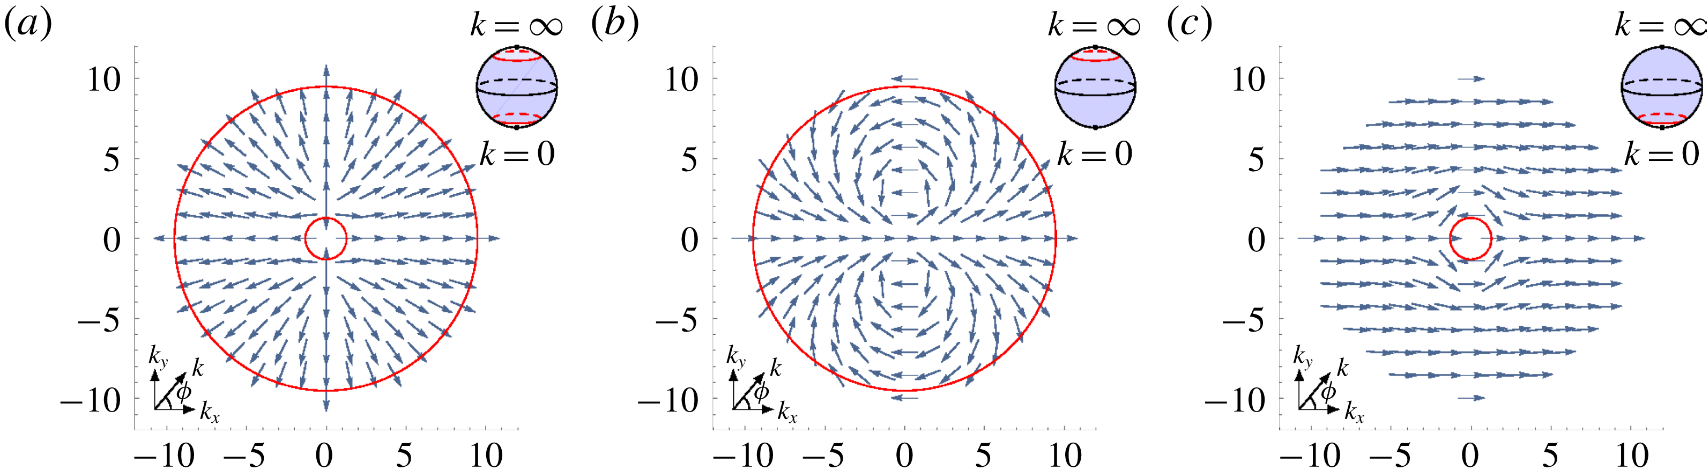
\includegraphics[width=16cm]{fig2.png}  %需调整
    \caption{(a)是$\psi_+$第二个分量的分布;(b)$\psi_+^A$,(c)$\psi_+^B$第二个分量的分布}
    \label{fig:2}
\end{figure}

接下来,通过一系列微分拓扑方面的讨论,
文章给出了计算Chern数的积分方法\cite{nakahara2003geometry},
经过简化有:
\begin{equation}
    C_+ = \dfrac{1}{2\pi} \int_0^{2\pi}  \dd \phi \, (\mathbf A_+^A - \mathbf A_+^B) \cdot  \mathbf e_\phi= \text{sign}(f) + \text{sign}(\epsilon) \ .
\end{equation}
文章指出如果由$\epsilon=0$出发推导Chern数会得到不合理的结论。

\subsection{零、负分支的拓扑}
负分支出于对称性,有$C_-=-C_+$。
同时由于零分支的特征向量在$\mathbb{R} \cup \{\infty\}$上是连续的,
可知其Chern数$C_0=0$。这样,改变不同的$f,\epsilon$就会有
不同的拓扑,因此考虑在空间上将两个不同拓扑的区域粘接起来,
得到一个间断界面。

\subsection{界面波}

在$y=0$设为界面,上方$f>0$,而下方$-f<0$。
经典的模型中$f$是线性分布的,因此符号是不同的。
本文认为两个半平面中$f$都是常数。
这个设置可见图\ref{fig:3}。

\begin{figure}[H]
    \centering
    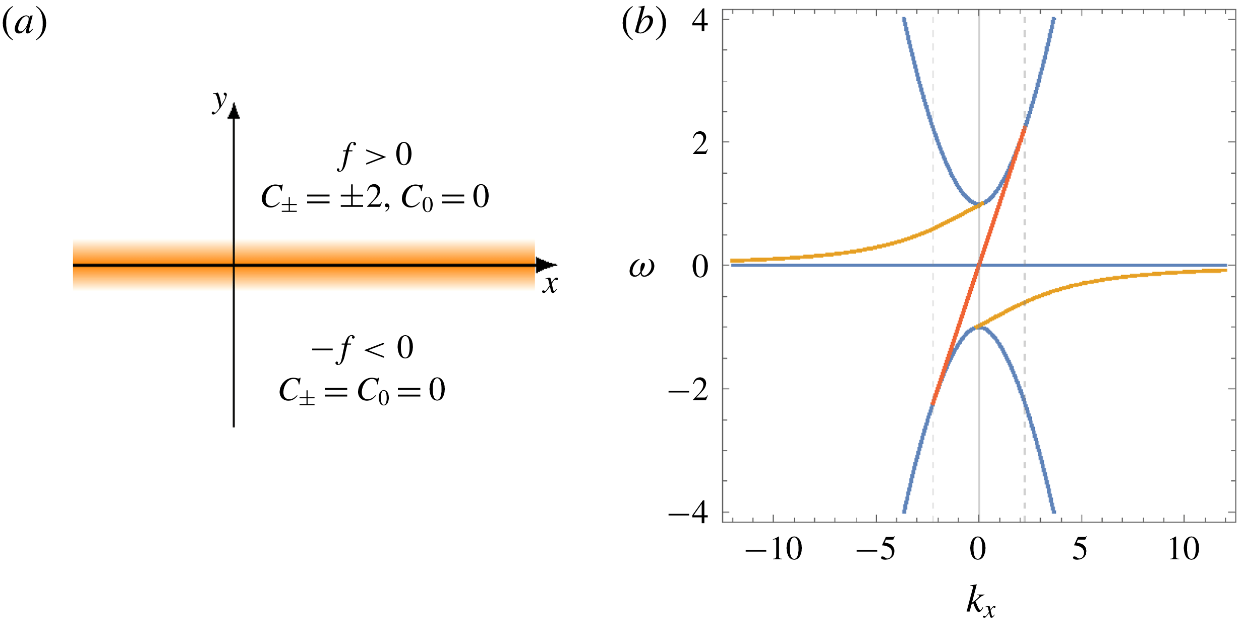
\includegraphics[width=16cm]{fig3.png}  %需调整
    \caption{(a)上下分界和赤道设置示意;(b)界面上的色散关系,橙色是Yanai类型的波,红色是Kelvin类型,
        蓝色是体波,其中$f=1,\epsilon=0.2$}
    \label{fig:3}
\end{figure}

考虑纬向的模态,
$(\eta, u, v) = \ee^{\ii (\omega t -k_x x)}(\tilde \eta, \tilde u, \tilde v)$,
等号右边的向量与$y,k_x,\omega$都有关。将其代入系统,
下文都省略右侧的波浪线有:
\begin{align}
    \ii \omega \eta & = \ii k_x u - \partial_y v \label{eq:first}                                        \\
    \ii \omega u    & = \ii k_x \eta + (\pm f - \epsilon  k_x^2) v + \epsilon  \partial_{yy} v           \\
    \ii \omega v    & = -\partial_y \eta - (\pm f - \epsilon  k_x^2) u - \epsilon  \partial_{yy} u  \, .
\end{align}
系统其实是非独立的,可消去$\eta$,化简为:
\begin{align}
    \label{eq:interface_ode_v}\big(\epsilon  \partial_{yy}  - \dfrac{k_x}{\omega} \partial_y  + (\pm f - \epsilon  k_x^2)\big)v & = \dfrac{\ii}{\omega}(\omega^2-k_x^2) u          \\
    \label{eq:interface_ode_u}\big(\epsilon  \partial_{yy}  + \dfrac{k_x}{\omega} \partial_y  + (\pm f - \epsilon  k_x^2)\big)u & = -\dfrac{\ii}{\omega}(\partial_{yy}+\omega^2) v
\end{align}
界面处施加界面连续条件:
\begin{equation}\label{eq:interface_gluing}
    u|_{y=0^-} = u|_{y=0^+}, \quad v|_{y=0^-} = v|_{y=0^-}, \quad \partial_y u|_{y=0^-} = \partial_y u|_{y=0^+}, \quad \partial_y v|_{y=0^-} = \partial_y v|_{y=0^-}
\end{equation}

为了寻求界面附近的解,设:
\begin{equation}
    u(y) = \left\lbrace \begin{array}{ll}
        u_\uparrow(y),   & y>0, \\
        u_\downarrow(y), & y<0, \\
    \end{array}\right.
\end{equation}
对$v$进行类似分解,进行进一步求解即可得到图\ref{fig:3}的关系。

\subsubsection{紧支化Kelvin波}

经过一系列推导,当$k_x=\omega$,且设$v\equiv 0$,
可给出
\begin{equation}\label{eq:q_up}
    u_\uparrow(y) = A_\uparrow \ee^{q_{\uparrow+} y} + B_\uparrow \ee^{q_{\uparrow-} y}
    \quad
    \text{where}
    \quad
    q_{\uparrow\pm} = - \dfrac{1}{2\epsilon } \big(\dfrac{k_x}{\omega} \pm \sqrt{1+4\epsilon (\epsilon k_x^2-f)}\big)
\end{equation}
这在$f\epsilon\leq 1/4$时是有意义的。定义$k_0=\sqrt{f/\epsilon}$,
为保证解在$y->\infty$是趋于0,要保证指数上的系数小于0,因此要求:
\begin{equation}
    u_\uparrow(y) = \left\lbrace \begin{array}{ll}
        A_\uparrow \ee^{q_{\uparrow+} y} + B_\uparrow \ee^{q_{\uparrow-} y}, & |k_x| < k_0,    \\
        A_\uparrow \ee^{q_{\uparrow+} y},                                    & |k_x| \geq k_0.
    \end{array}\right.
\end{equation}
相似在下半平面有
\begin{equation}\label{eq:q_down}
    q_{\downarrow\pm} = - \dfrac{1}{2\epsilon } \big(\dfrac{k_x}{\omega} \pm \sqrt{1+4\epsilon (\epsilon k_x^2+f)}\big)
\end{equation}。
进一步考虑$u_\downarrow$的有界性和边界条件的实施,可得:
\begin{equation}\label{u_kelvin}
    u(y) = \left\lbrace \begin{array}{lll}
        A_\uparrow \Big(\ee^{q_{\uparrow+} y} -\dfrac{q_{\uparrow+}-q_{\downarrow-}}{q_{\uparrow-}-q_{\downarrow-}} \ee^{q_{\uparrow-} y} \Big) & y>0,          & |k_x|<k_0 \\
        A_\uparrow \dfrac{q_{\uparrow-}-q_{\uparrow+}}{q_{\uparrow-}-q_{\downarrow-}}\ee^{q_{\downarrow-} y}                                    & y<0,          & |k_x|<k_0 \\
        0                                                                                                                                       & |k_x|\geq k_0
    \end{array}\right.
\end{equation}
文章指出在$\epsilon\rightarrow 0$时,可发现这个解与经典的Kelvin波是一致的。

\subsubsection{紧支化Yanai波}
此时假设$k^2_x\neq\omega^2$且$v\neq 0$,则有关于$v$的方程,
在上半平面内
\begin{equation}\label{eq:yanai_v_order4}
    \Big(\epsilon ^2 \partial^{(4)}_{y}  + (2\epsilon ( f-\epsilon  k_x^2)-1) \partial^{(2)}_{y} + ( f-\epsilon  k_x^2))^2-(\omega^2-k_x^2)\Big)v = 0
\end{equation}
对应代数方程有根
\begin{equation}\label{eq:def_Spm}
    S_\pm = \dfrac{1}{2\epsilon ^2} \Big( 1+2\epsilon (\epsilon  k_x^2- f) \pm \sqrt{1+4 \epsilon  (\epsilon  \omega^2-f)} \Big)
\end{equation}
其中$s^2=S_\pm$,则为了有非平凡模态要求$S_\pm>0$,则有:
\begin{equation}\label{eq:interface_bulk_limit}
    \Delta(k_x,\omega) := k_x^2-\omega^2 + (f-\nu k_x^2)^2 > 0
\end{equation}、
此时有四个实根:
\begin{equation}
    s_{\uparrow1} = \sqrt{S_+}, \quad s_{\uparrow2} = \sqrt{S_-}, \quad s_{\uparrow3} = -\sqrt{S_+}, \quad s_{\uparrow4} = -\sqrt{S_-}
\end{equation}
计算$s_{\downarrow1,...4}$类似,只需将$f$代换为$-f$。

接下来经过一系列推导,本文给出了一个隐式的色散关系:
\begin{equation}\label{eq:Yanai_implicit}
    \epsilon ^2(s_{\downarrow 1}-s_{\uparrow 3})(s_{\downarrow 2}-s_{\uparrow 3})(s_{\downarrow 1}-s_{\uparrow 4})(s_{\downarrow 2}-s_{\uparrow 4}) + 2 f \dfrac{k_x}{\omega} (s_{\downarrow 1}+ s_{\downarrow 2}-s_{\uparrow 3} - s_{\uparrow 4}) - 4 f^2 = 0
\end{equation}
这个色散关系可以数值求解,得到如图\ref{fig:3}中的结果。
同时,可验证$\epsilon\rightarrow0$时有经典的Yanai波。

文章表示$v\neq0, k_x^2=\omega^2$的情景的推导比较繁琐,但是没有额外的模态出现。

\section{关于体-面相似性的进一步讨论}

文章对体-边相似性进一步讨论。
文章给出了有边界条件的模态数值解,边界条件有无滑移或者无穿透两种,
如图\ref{fig:4}。

\begin{figure}[H]
    \centering
    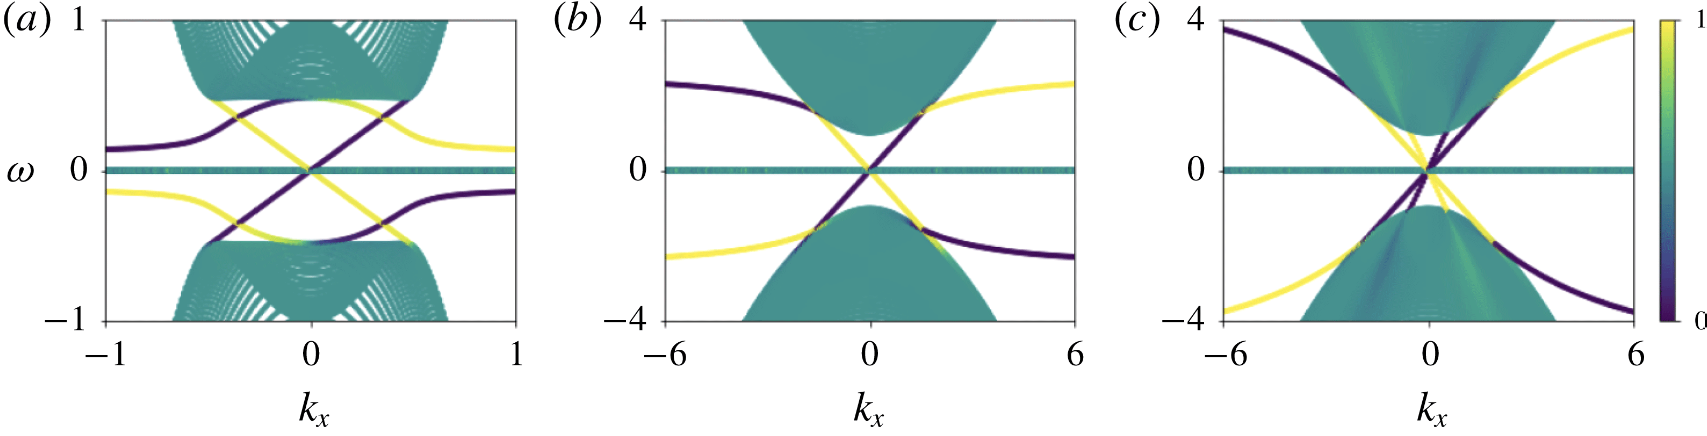
\includegraphics[width=16cm]{fig4.png}  %需调整
    \caption{(a)是$f=1,\epsilon=4$,无滑移边界条件计算的色散关系;
        (b)是$f=1,\epsilon=0.2$,无滑移边界条件计算的色散关系;
        (c)是(b)改为无穿透条件的结果;图中不同颜色代表不同的y位置}
    \label{fig:4}
\end{figure}

文章发现,考虑$y=0$的情况(蓝色线条),
数值结果中图\ref{fig:4}(a)对于固定的频率一般有两个模态,与文章的分析一致;
然而在$\omega$很小或者$\epsilon$减小后,就可能变成一个模态;
同时如果改变边界条件如(c)中,就可以出现三个模态。文章中解析计算
的情况是粘合两个区域得来的,在这种情况下刚好可以得到体-面相似性的结论。

\section{结论}
文章研究的内容可以看成是对经典赤道波理论模型的推广,
其中的$f$不是线性分布而是有一个间断变化。
本文假设在两个半平面中$f$是常数。
经过理论分析,本文发现在这样的模型下,与经典理论不同,
不是所有的模态都约束在赤道线上,而只有Kelvin波和Yanai类型的波
被约束在赤道线上;其他波都不是局部的。而且,其中没有Rossby波。
在这一系列推导中,本文从拓扑角度出发,通过粘合两个拓扑指标不同的
区域解释了一些性质的拓扑由来。本文的分析表明,Yanai波应该被认为是
混合地转-重力波而非混合Rossby-重力波,因为Yanai波可以在没有
Rossby波的情况下存在。本文的模型依赖于一个正则项odd viscosity的使用,
但是极限分析表明当正则项趋于0可以还原经典解。

总之,本文在一个简化的赤道波模型中,通过理论分析给出了一系列
有体-面相似性的模态结论,成为了一个很简单的可解的流体中体-面相似性的案例。
同时,由于尖锐间断的存在,本文的研究有助于进一步理解有边界条件的情况下的
体-面相似性。

\section{阅读体会与感悟}
本文的研究内容是浅水方程的波,其与三维流体中的二维波动有很类似的求解思路。
当求解体波的时候,是二维波动问题;而求解界面附近的波时,
加入的模态就是一维的。特别是一维模态中的Kelvin波、Yanai波
的形式都与三维无粘不可压流体界面上的线性波形式非常相似。
同时,在考虑界面条件时,虽然不同,本文使用的界面连续条件也
与无粘不可压流体的界面波的情况有很大的相似之处。
和课程中一样,文章最后也得到了一系列色散关系作为
分析结果。
因此,从波动力学的角度上看,本文与传统的流体波动
求解过程非常相近。

当然,另一方面看,本文需要讨论体-面相似性,
这是一个拓扑上的定义,因此需要
引入一些微分拓扑的计算,和构造。
这些工具与物理学的很多方面有所借鉴,
这体现了现代数学工具和领域间交叉融合的一些特点。

本文研究一方面可以如文中所说,进一步研究边界条件对波动带来的影响;
另一方面可以考虑在方程中引入更多非线性,研究波动力学系统的非线性特性。
同时,也可以考虑与实验结合更加紧密,在合适的条件下观测理论上给出的波。



\bibliography{refs}{}
\bibliographystyle{unsrt}

% \section*{附录}
% 本文计算代码都在\href{https://github.com/harryzhou2000/HW_ACFD}{Github Repo中(点击访问)}。































% \section{SECTION 节}

% 一个

% \subsection{SUBSECTION 小节}

% 示例

% \subsubsection{SUBSUBSECTION 小节节}

% 字体字号临时调整:
% {
%    \sffamily\bfseries\zihao{3} 哈哈哈哈哈 abcde %三号 sans系列字体(一开始设置的) 加粗
%    %只对大括号范围内的后面的字有用,在标题、题注里面同样
% }
% { 
%    \CJKfamily{kaiti}\zihao{5}\itshape 哈哈哈哈哈 abcde%三号 kaiti(一开始设置的, 斜体(英文有变)
%    %只对大括号范围内的后面的字有用,在标题、题注里面同样
% }

% 一大堆一大堆一大堆一大堆一大堆一大堆一大堆一大堆一大堆一大堆
% 一大堆一大堆一大堆一大堆一大堆一大堆一大堆一大堆一大堆一大堆一大堆一大堆
% 一大堆一大堆一大堆一大堆一大堆一大堆一大堆一大堆一大堆一大堆一大堆一大堆
% 一大堆一大堆一大堆一大堆一大堆一大堆一大堆一大堆一大堆一大堆一大堆一大堆

% \begin{center}
%     居中的什么乱七八糟东西
% \end{center}


% 一个列表:
% \begin{itemize}
%     \item asef
%     \item[\%] asdf
%     \item[\#] aaa
% \end{itemize}

% 一个有序列表:
% \begin{enumerate}
%     \item asef
%     \item[\%\%] asdf
%     \item aaa
% \end{enumerate}

% 一个嵌套列表,考虑缩进:
% \begin{enumerate}[itemindent=2em] %缩进
%     \item asef \par asaf 东西东西东西东西东西东西东西东西东西东西东西东西东西东西东西东西东西东西东西东西东西东西东西东西,
%           F不是不是不是不是不是不是不是不是不是不是不是不是不是不是不是
%           \begin{itemize}[itemindent=2em]  %缩进
%               \item lalala
%               \item mamama
%           \end{itemize}
%     \item asdf
%     \item aaa
% \end{enumerate}

% \section{SECTION}

% 图片排版:

% \begin{figure}[H]
%     \begin{minipage}[c]{0.45\linewidth}  %需调整
%         \centering
%         \includegraphics[width=8cm]{RAM_O2_4660.png}  %需调整
%         \caption{第一个图}
%         \label{fig:a}
%     \end{minipage}
%     \hfill %弹性长度
%     \begin{minipage}[c]{0.45\linewidth}  %需调整
%         \centering
%         \includegraphics[width=8cm]{RAM_O4_4660.png}  %需调整
%         \caption{第二个图}
%         \label{fig:b}
%     \end{minipage}
% \end{figure}

% figure的选项为“htbp”时,会自动浮动,是“H”则和文字顺序严格一些。

% \begin{figure}[H]
%     \begin{minipage}[c]{0.45\linewidth}  %需调整
%         \centering
%         \includegraphics[width=8cm]{RAM_O2_4660.png}  %需调整
%         \label{fig:x}
%     \end{minipage}
%     \hfill %弹性长度
%     \begin{minipage}[c]{0.45\linewidth}  %需调整
%         \centering
%         \includegraphics[width=8cm]{RAM_O4_4660.png}  %需调整
%         \label{fig:y}
%     \end{minipage}
%     \caption{第三个图}
% \end{figure}

% \begin{figure}[H]
%     \centering
%     \includegraphics[width=8cm]{RAM_O4_4660.png}  %需调整
%     \label{fig:c}
%     \caption{第四个图}
% \end{figure}



% \subsection{SUBSECTION}

% 关于怎么搞表格:

% \begin{table*}[htbp]
%     \footnotesize
%     \begin{center}
%         \caption{一端力矩载荷下的结果\fontsize{0pt}{2em}} %需要学习统一设置;0代表不变?
%         \label{表2}
%         \begin{tabular}{|c|c|c|c|c|c|c|}
%             \hline
%             节点数                              & 积分方案              & 单元数                & $h=1m$                & $h=0.1m$              & $h=0.05m$             & $h=0.01m$             \\
%             \hline
%             \multirow{6}{*}{2}                  & \multirow{3}{*}{精确} & 1                     & 4.235294117647059E-08 & 1.406250000000000E-06 & 2.862823061630218E-06 & 1.439654482924097E-05 \\
%             \cline{3-7}
%                                                 &                       & 10                    & 5.975103734439814E-08 & 4.235294117646719E-05 & 1.800000000000410E-04 & 1.406249999999849E-03 \\
%             \cline{3-7}
%                                                 &                       &
%             10000                               & 5.999999915514277E-08 & 5.999996622448291E-05 & 4.799989509752562E-04 & 5.999793702477535E-02                                                 \\
%             \cline{2-7}
%                                                 & \multirow{3}{*}{减缩} & 1                     & 6.000000000000001E-08 & 5.999999999999972E-05 & 4.799999999999911E-04 & 6.000000000003492E-02 \\
%             \cline{3-7}
%                                                 &                       & 10                    & 6.000000000000071E-08 & 5.999999999999142E-05 & 4.799999999995399E-04 & 5.999999999903294E-02 \\
%             \cline{3-7}
%                                                 &                       & 10000                 & 6.000000112649221E-08 & 5.999999234537814E-05 & 4.799997501925065E-04 & 6.000037607984510E-02 \\
%             \hline

%             \multirow{6}{*}{3}                  & \multirow{3}{*}{精确} & 1                     & 6.000000000000003E-08 & 6.000000000000202E-05 & 4.800000000000831E-04 & 6.000000000056749E-02 \\
%             \cline{3-7}
%                                                 &                       & 10                    & 5.999999999999932E-08 & 6.000000000004190E-05 & 4.800000000000206E-04 & 6.000000001613761E-02 \\
%             \cline{3-7}
%                                                 &                       & 10000                 & 6.000000013769874E-08 & 5.999989495410481E-05 & 4.799942099727246E-04 & 6.000263852944890E-02 \\
%             \cline{2-7}
%                                                 & \multirow{3}{*}{减缩} & 1                     & 6.000000000000002E-08 & 6.000000000000267E-05 & 4.800000000000754E-04 & 5.999999999989982E-02 \\
%             \cline{3-7}
%                                                 &                       & 10                    & 5.999999999999899E-08 & 5.999999999987338E-05 & 4.799999999947916E-04 & 5.999999998625345E-02 \\
%             \cline{3-7}
%                                                 &                       & 10000                 & 5.999999728157785E-08 & 5.999994914321980E-05 & 4.800008377474699E-04 & 5.999472246346305E-02 \\
%             \hline

%             \multicolumn{3}{|c|}{欧拉-伯努利解} & 6.000000000000000E-08 & 6.000000000000000E-05 & 4.800000000000000E-04 & 6.000000000000000E-02                                                 \\
%             \hline
%         \end{tabular}
%     \end{center}
% \end{table*}

% 多行、多列表格的示例,基本思想是,多列的那个东西放在多列的最上面一格,下面的行要用\&来空开,也就是\&的数目
% 和普通表格一样,是列数减一;
% 多列的部分的话,就是每行内的操作,相应的\&就少了,见最后一行。

% tabular的“|c|c|c|c|c|c|c|”,意思是,竖线-居中-竖线-居中-竖线……,可以选择省略一些竖线;
% 每行之间的hline,代表贯通的横线,cline是有范围的横线。

% \subsubsection{SUBSUBSECTION}

% newcommand可以用来定义新指令,似乎基本上就是字符串替换……不太懂,总之在公式里面可以用,
% 外面也经常用。






% 公式这么写:
% \begin{equation}
%     \begin{aligned}
%         \frac{aa(x^1+x^2)}{\sqrt{x^1x^2}}
%         \nabla\times\uu
%         = & u_{j;m}\g^m\times\g^j
%         =u_{j;m}\epsilon^{mjk}\g_k
%         =u_{j,m}\epsilon^{mjk}\g_k                           \\
%         = & \frac{1}{\sqrt{g}}\left|
%         \begin{matrix}
%             \g_1       & \g_2       & \g_3       \\
%             \partial_1 & \partial_2 & \partial_3 \\
%             u_1        & u_2        & u_3
%         \end{matrix}
%         \right|
%         =\frac{\sqrt{x^1x^2}}{aa(x^1+x^2)}
%         \left|
%         \begin{matrix}
%             \g_1                        & \g_2                        & \g_3       \\
%             \partial_1                  & \partial_2                  & \partial_3 \\
%             u^1\frac{a^2(x^1+x^2)}{x^1} & u^2\frac{a^2(x^1+x^2)}{x^2} & u^3
%         \end{matrix}
%         \right|                                              \\
%         = & \frac{\sqrt{x^1x^2}}{aa(x^1+x^2)}
%         [[\g_1\,\g_2\,\g_3]]
%         diag\left(
%         u^3_{,2}-u^2_{,3}\frac{a^2(x^1+x^2)}{x^2},\,
%         u^1_{,3}\frac{a^2(x^1+x^2)}{x^1}-u^3_{,1},\, \right. \\
%           & \left.
%         u^2_{,1}\frac{a^2(x^1+x^2)}{x^2}+u^2\frac{a^2}{x^2}
%         -
%         u^1_{,2}\frac{a^2(x^1+x^2)}{x^1}-u^1\frac{a^2}{x^1}
%         \right)                                              \\
%         = & \frac{\sqrt{x^1x^2}}{aa(x^1+x^2)}
%         [[\bm{e}_1\,\bm{e}_2\,\bm{e}_3]]
%         \left[\begin{array}{ccc} a & -a & 0\\ \frac{a\,x^{2}}{\sqrt{x^{1}\,x^{2}}} & \frac{a\,x^{1}}{\sqrt{x^{1}\,x^{2}}} & 0\\ 0 & 0 & 1 \end{array}\right]              \\
%           & diag\left(
%         u^3_{,2}-u^2_{,3}\frac{a^2(x^1+x^2)}{x^2},\,
%         u^1_{,3}\frac{a^2(x^1+x^2)}{x^1}-u^3_{,1},\, \right. \\
%           & \left.
%         u^2_{,1}\frac{a^2(x^1+x^2)}{x^2}+u^2\frac{a^2}{x^2}
%         -
%         u^1_{,2}\frac{a^2(x^1+x^2)}{x^1}-u^1\frac{a^2}{x^1}
%         \right)
%     \end{aligned}
%     \label{eq:curlu}
% \end{equation}

% 如果不想带编号的公式(或者图表),用 equation* 这种环境。

% 引用,如果是引用的图表,就用表\ref{表2},图\ref{fig:a}这种,代码里是用label定义的标签来引用,
% 编号是自动生成的。公式引用一般写成:\eqref{eq:curlu}。目前这些引用自动会有超链接,反正有那个包自动
% 好像就会有……呜呜呜也不知道是怎么做到的,先这么用吧。

% \paragraph{PARA}

% 引用文献用\\cite这些,要用bibtex,暂时不做。

% \subparagraph{SUBPARA}

\end{document}